\documentclass[11pt]{article}
\setlength{\topmargin}{-1.5cm}
\setlength{\textheight}{23cm}
\setlength{\oddsidemargin}{0mm}
\setlength{\evensidemargin}{0mm}
\setlength{\textwidth}{17cm}
\usepackage{graphicx, color}
\usepackage{amsmath, amssymb, amsthm}
\usepackage{enumerate}
\usepackage{hyperref}

\newcommand{\noin}{\noindent}

\newcommand{\Var}{\text{Var}}


\begin{document}
\noindent {\large  \textbf{Shawn Pan -- Stat 139 Homework 5, Fall 2016}} \medskip

\noindent \textbf{Problem 1.}

\begin{align*}
\textrm{Mean texts by underclassmen}&: \> \mu_{und}\\
\textrm{Mean texts by upperclassmen}&: \> \mu_{up}\\
H_0&: \mu_{und} - \mu_{up} = 0\\
H_A&: \mu_{und} - \mu_{up} \ne 0
\end{align*}

We assume the samples are independent.  We also assume the two distributions are the same to make a statement about the means.  We randomly sample 100,000 permutations and get the following reference distribution:

\begin{figure}[h!]
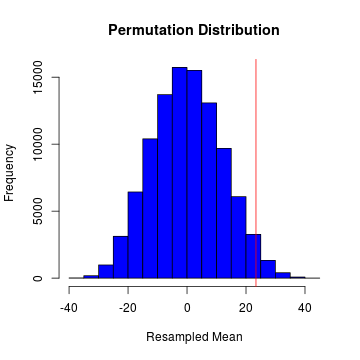
\includegraphics[width=3in]{permutations.png}
\end{figure}

Our p-value is 0.0512.  At an $\alpha = 0.05$ level, we do not have enough evidence to conclude the mean number of texts sent by underclassmen is different from the mean number of texts sent by upperclassmen.

\pagebreak


\noindent {\bf Problem 2.}

\vspace{0.1in}

\noindent (a) Increasing the sample size will increase the power of the test, because the standard deviation of the means will go down, so the distributions of the null and alternative will be tighter and overlap less.

\vspace{0.1in}

\noindent (b) Decreasing the effect size will decrease the power, because the null and alternative distributions will be shifted closer together and overlap more.

\vspace{0.1in}

\noindent(c) Increasing the standard deviation will decrease the power, because the distributions of the null and alternative will be wider and overlap more.

\vspace{0.1in}

\noindent (d)

\begin{align*}
\alpha &= 0.05\\
1 - \beta &= 0.8\\
\sigma &= 18\\
\mu_A - \mu_0 &= 5\\
n &\ge \left(\frac{\sigma (|z_{1-\alpha/2}| + |z_{1-\beta}|)}{\mu_A - \mu_0} \right)^2 = 102
\end{align*}

\begin{verbatim}
ceiling((18 * (qnorm(0.975) + qnorm(0.8)) / 5)^2)
[1] 102
\end{verbatim}

We need $n \ge 102$ to get 80\% power.

\vspace{0.3in}


\noindent {\bf Problem 3.}

\vspace{0.1in}

\noindent (a)

\begin{align*}
H_0&: \bar{Y}_{trt} - \bar{Y}_{ctrl} = 0\\
H_A&: \bar{Y}_{trt} - \bar{Y}_{ctrl} \ne 0
\end{align*}

The means will be normally distributed with variance $\frac{\sigma^2}{n}$.

\begin{align*}
\bar{Y}_{trt} &\sim N(\mu+\delta,\frac{\sigma^2}{n_{trt}})\\
\bar{Y}_{ctrl} &\sim N(\mu,\frac{\sigma^2}{n_{ctrl}})
\end{align*}

When you subtract two independent normal distibutions, you get another normal distribution.

Null difference distribution and z-statistic:
\begin{align*}
(\bar{Y}_{trt} - \bar{Y}_{ctrl}) &\sim N(0, \frac{\sigma^2}{n_{trt}} + \frac{\sigma^2}{n_{ctrl}})\\
z_0 &= \frac{(\bar{Y}_{trt} - \bar{Y}_{ctrl}) - 0}{\sqrt{\frac{\sigma^2}{n_{trt}} + \frac{\sigma^2}{n_{ctrl}}}}
\end{align*}

Alternative difference distribution and z-statistic:
\begin{align*}
(\bar{Y}_{trt} - \bar{Y}_{ctrl}) &\sim N(\delta, \frac{\sigma^2}{n_{trt}} + \frac{\sigma^2}{n_{ctrl}})\\
z_A &= \frac{(\bar{Y}_{trt} - \bar{Y}_{ctrl}) - \delta}{\sqrt{\frac{\sigma^2}{n_{trt}} + \frac{\sigma^2}{n_{ctrl}}}}
\end{align*}

\vspace{0.1in}

\noindent (b)

\begin{align*}
z_0 &= z_{1-\alpha/2} \quad \textrm{(cutoff for null)}\\
z_A &= z_{\beta} \quad \textrm{(cutoff for alternative)}\\
z_0 - z_A &= z_{1-\alpha/2} - z_\beta\\
\frac{\delta}{\sqrt{\frac{\sigma^2}{n_{trt}} + \frac{\sigma^2}{n_{ctrl}}}} &= z_{1-\alpha/2} - z_\beta\\
\delta &= (z_{1-\alpha/2} - z_\beta)\sqrt{\frac{\sigma^2}{n_{trt}} + \frac{\sigma^2}{n_{ctrl}}}
\end{align*}

Note that $z_{1-\alpha/2}$ is positive and $z_\beta$ is negative.  Alternatively, we can add the absolute values.

\vspace{0.1in}

\noindent (c)

\begin{align*}
\frac{\delta}{(z_{1-\alpha/2} - z_\beta)} &= \sigma \sqrt{\frac{2}{n}}\\
\sqrt{n} &= \frac{\sqrt{2}\sigma(z_{1-\alpha/2} - z_\beta)}{\delta}\\
n &= 2\left( \frac{\sigma (z_{1-\alpha/2} - z_\beta)}{\delta} \right)^2
\end{align*}

\vspace{0.1in}

\noindent (d)

\begin{align*}
n &\ge 2\left( \frac{5 (z_{1-\alpha/2} - z_\beta)}{18} \right)^2\\
n &\ge 204
\end{align*}

\begin{verbatim}
ceiling(2 * (18 * (qnorm(0.975) - qnorm(0.2)) / 5)^2)
[1] 204
\end{verbatim}

We need 204 patients per group for a total of 408 patients.

\vspace{0.1in}

\noindent (e) The total number of patients has increased because we need test patients for both groups and the variance has increased because we are estimating the control group mean in addition to the treatment group mean.

\pagebreak


\noindent {\bf Problem 4.}

\noindent (a)

$$\binom{16}{2} = \frac{16!}{14!2!} = \frac{(16)(15)}{2} = 120$$

\vspace{0.1in}

\noindent (b)

We perform an unpooled t-test.  The null hypothesis is that the difference in mean voter gap between LA Times and NBC News is zero.  The alternative hypothesis is that the difference is non-zero.

\begin{verbatim}
data:  gap_la and gap_nbc
t = -7.1276, df = 20.354, p-value = 5.972e-07
95 percent confidence interval:
 -10.755760  -5.889695
\end{verbatim}

At a $\alpha = 0.05$ level, we reject the null hypothesis and conclude that the LA Times polls show a lower voter gap than NBC News.  We are 95\% confident that the difference between the mean voter gaps (LA Times - NBC News) is between -10.76 and -5.89.

\vspace{0.1in}

\noindent (c)

\begin{verbatim}
diff <- mean(gap_la) - mean(gap_nbc)
se <- sqrt(var(gap_la) / length(gap_la) + var(gap_nbc) / length(gap_nbc))
tstar <- qt(0.025 / 120, df)
tstar
diff + tstar * se
diff - tstar * se
\end{verbatim}

We adjust $\alpha^* = \frac{\alpha}{120}$ and get a critical t-value of $t^* = 4.21$.  We are 95\% confident that the difference between the mean voter gaps (LA Times - NBC News) is between -13.24 and -3.41.  The confidence interval is wider than the unadjusted interval, but our conclusions have not changed.

\vspace{0.1in}

\noindent (d)

\begin{verbatim}
tstar <- qtukey(0.95, 16, 113 - 16) / sqrt(2)
tstar
diff + tstar * se
diff - tstar * se
\end{verbatim}

Note that we have $I = 16$ groups and $n = 113$ polls (ignoring the 4 in the Other category).  We get a critical value of $3.52$.  We are 95\% confident that the difference between the mean voter gaps (LA Times - NBC News) is between -12.43 and -4.22.

The Tukey approach produces a narrower interval than the more conservative Bonferroni approach.  However, the variances of voter gap range from 2.7 for Economist/YouGov to 37.3 for McClatchy/Marist.  The Tukey approach is not appropriate, because the equal variances assumption is violated.

\pagebreak

\noindent {\bf Problem 5.}

\noindent (a)

\begin{align*}
I &= 4\\
n &= 117\\
df_T &= 117 - 1 = 116\\
df_B &= I - 1 = 3\\
df_W &= n - I = 113\\
\bar{Y} &= \frac{32(3.031) + 25(6.240) + 35(2.886) + 25(6.280)}{117} = 4.368\\
SSB &= 32(3.031 - 4.368)^2 + 25(6.240 - 4.368)^2 + 35(2.886 - 4.368)^2 + 25(6.280 - 4.368)^2 = 313\\
SSW &= (32 - 1)(4.468)^2 + (25 - 1)(3.153)^2 + (35 - 1)(3.394)^2 + (25 - 1)(3.824)^2 = 1600\\
SST &= 313 + 1600 = 1913\\
S^2_B &= 313 / 3 = 104\\
S^2_W &= 1600 / 113 = 14\\
S^2 &= 1913 / 116 = 16.5\\
F &= 104 / 14 = 7.4
\end{align*}

\begin{center}
  \begin{tabular}{lllll}
Source & SS & DF & MS & F\\
Between & 313 & 3 & 104 & 7.4\\
Within & 1600 & 113 & 14 &\\
Total & 1913 & 116 & 16.5
  \end{tabular}
\end{center}

\vspace{0.1in}

\noindent (b)

Our null hypothesis is that mean voter gaps in all four months is equal.  Our alternative hypothesis is that there is a difference between some combination of the means.

\begin{verbatim}
            Df  Sum Sq Mean Sq F value    Pr(>F)
data$month   3  313.08  104.36    7.37 0.0001484 ***
Residuals  113 1600.11   14.16
\end{verbatim}

At the $\alpha = 0.05$ level, we reject the null hypothesis and conclude there is a difference between some combination of the monthly means of voter gap.

\pagebreak

\noindent (c) We will use the Tukey-Kramer procedure, because we want to do all pairwise comparisons and the equal variances assumption is reasonable $(4.468/3.153)^2 \approx 2$.

\begin{verbatim}
                   diff        lwr        upr     p adj
7-Jul-10-Oct -3.2487500 -5.8680294 -0.6294706 0.0085739
8-Aug-10-Oct -0.0400000 -2.8154562  2.7354562 0.9999808
9-Sep-10-Oct -3.3942857 -5.9638589 -0.8247126 0.0044075
8-Aug-7-Jul   3.2087500  0.5894706  5.8280294 0.0096869
9-Sep-7-Jul  -0.1455357 -2.5455718  2.2545004 0.9985842
9-Sep-8-Aug  -3.3542857 -5.9238589 -0.7847126 0.0050253
\end{verbatim}

At the $\alpha = 0.05$ level significant differences occur between the mean voter gaps in the following pairs: Jul/Oct, Sep/Oct, Aug/Jul, and Sep/Aug

\vspace{0.1in}

\noindent (d) We perform a contrast t-test.

\begin{align*}
a &= (\frac{32}{92}, \frac{25}{92}, \frac{35}{92}, -1)\\
\psi &= \frac{32}{92}\mu_7 + \frac{25}{92}\mu_8 + \frac{35}{92}\mu_9 - \mu_{10}\\
H_0&: \psi = 0\\
H_A&: \psi \ne 0\\
T &= \frac{\frac{32}{92}\bar{x}_7 + \frac{25}{92}\bar{x}_8 + \frac{35}{92}\bar{x}_9 - \bar{x}_{10}}{\sqrt{14.16}\sqrt{a^2/n}}\\
T &= -2.87
\end{align*}

We get a t-statistic of -2.87 which corresponds to a two-sided p-value of 0.005 on a t-distribution with 113 degrees of freedom.  At the $\alpha = 0.05$ level, we have evidence that the voter gap is greater in October than July, August, and September combined.

\vspace{0.1in}

\noindent (e)

\begin{verbatim}
           Df Sum Sq Mean Sq F value    Pr(>F)
data$month  3 313.08 104.362 12.0711 8.810e-07 ***
data$poll  16 761.49  47.593  5.5049 3.484e-08 ***
Residuals  97 838.62   8.646
\end{verbatim}

\vspace{0.1in}

\noindent (f)

\begin{verbatim}
                     Df Sum Sq Mean Sq F value    Pr(>F)
data$month            3 313.08 104.362 12.8926 1.145e-06 ***
data$poll            16 761.49  47.593  5.8795 1.424e-07 ***
data$month:data$poll 34 328.65   9.666  1.1941    0.2672
Residuals            63 509.97   8.095
\end{verbatim}

\pagebreak

\noindent (g)

\begin{figure}[h!]
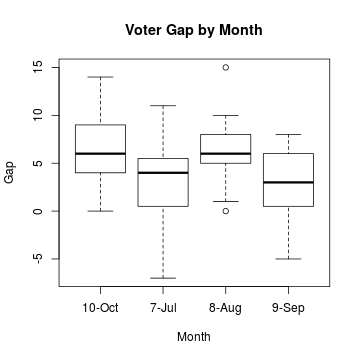
\includegraphics[width=3in]{boxplotmonth.png}
\end{figure}

\begin{figure}[h!]
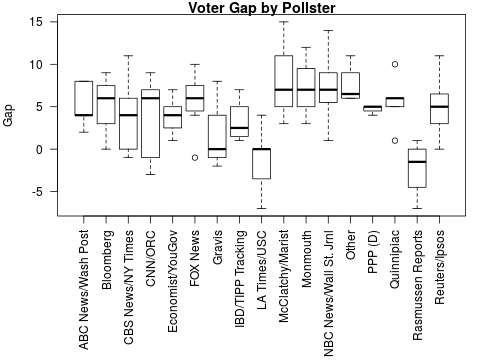
\includegraphics[width=4in]{boxplotpoll.png}
\end{figure}

\begin{figure}[h!]
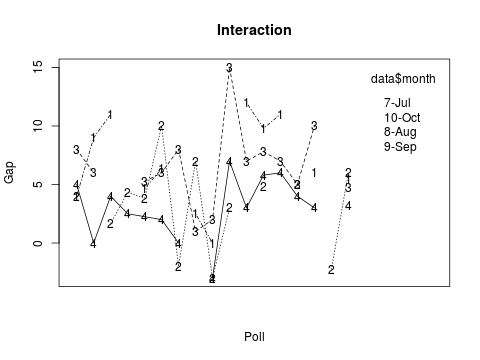
\includegraphics[width=4in]{interactions.png}
\end{figure}

\pagebreak

\noindent (h) The boxplot by month and our analysis in parts (b), (c), and (d) support the hypothesis that the voter gap varied by month.  The boxplot by pollster and the significant F-statistic in part (e) suggests voter gap is related to pollster controlling for month.  The interaction plot is very messy, because not all pollsters conducted polls each of the four months.  The interaction plot suggests there might be some interaction since the four lines are not equally spaced, but the p-value of 0.2672 in part (f) suggests we do not have enough evidence to support an interaction.

\end{document}